%%%%%%%%%%%%%%%%%%%%%%%%%%%%%%%%%%%%%%%%%
% Simple Sectioned Essay Template
% LaTeX Template
%
% This template has been downloaded from:
% http://www.latextemplates.com
%
% Note:
% The \lipsum[#] commands throughout this template generate dummy text
% to fill the template out. These commands should all be removed when 
% writing essay content.
%
%%%%%%%%%%%%%%%%%%%%%%%%%%%%%%%%%%%%%%%%%

%----------------------------------------------------------------------------------------
% PACKAGES AND OTHER DOCUMENT CONFIGURATIONS
%----------------------------------------------------------------------------------------

\documentclass[12pt]{article} % Default font size is 12pt, it can be changed here
\usepackage[utf8]{inputenc} % utf8 support
\usepackage[T1]{fontenc}

\usepackage{geometry} % Required to change the page size to A4
\geometry{a4paper} % Set the page size to be A4 as opposed to the default US Letter

\usepackage{graphicx} % Required for including pictures

% \usepackage{float} % Allows putting an [H] in \begin{figure} to specify the exact location of the figure
\usepackage{wrapfig} % Allows in-line images such as the example fish picture

\usepackage[style=numeric, backend=biber, sorting=none]{biblatex}
\bibliography{kilgarvan.bib}

\linespread{1.2} % Line spacing

%\setlength\parindent{0pt} % Uncomment to remove all indentation from paragraphs

\graphicspath{{./img/}} % Specifies the directory where pictures are stored

\newlength{\wideitemsep}
\setlength{\wideitemsep}{.5\itemsep}
\addtolength{\wideitemsep}{-7pt}
\let\olditem\item
\renewcommand{\item}{\setlength{\itemsep}{\wideitemsep}\olditem}

\begin{document}

%----------------------------------------------------------------------------------------
% TITLE PAGE
%----------------------------------------------------------------------------------------

\begin{titlepage}
  \newcommand{\HRule}{\rule{\linewidth}{0.5mm}} % Defines a new command for the horizontal lines, change thickness here

  \center % Center everything on the page

  \textsc{\LARGE University College Cork}\\[1.5cm] % Name of your university/college
  \textsc{\Large Wind Energy}\\[0.5cm] % Major heading such as course name
  % \textsc{\large Minor Heading}\\[0.5cm] % Minor heading such as course title

  \HRule \\[0.4cm]
  { \huge Kilgarvan Wind Farm Visit 28-10-2015}\\[0.5cm] % Title of your document
  \HRule \\[1.5cm]

  \begin{minipage}{0.4\textwidth}
  \begin{flushleft} \large
  \emph{Author:} Peter \textsc{Armstrong} \\% Your name 
  \emph{Student ID:} 115224113
  \end{flushleft}
  \end{minipage}
  ~
  \begin{minipage}{0.4\textwidth}
  \begin{flushright} \large
  % \emph{Supervisor:} \\
  % Dr. James \textsc{Smith} % Supervisor's Name
  \end{flushright}
  \end{minipage}\\[4cm]

  {\large \today}\\[3cm] % Date, change the \today to a set date if you want to be precise

  \vfill % Fill the rest of the page with whitespace

% itemize changes
\newlength{\wideitemsep}
\setlength{\wideitemsep}{.5\itemsep}
\addtolength{\wideitemsep}{-7pt}
\let\olditem\item
\renewcommand{\item}{\setlength{\itemsep}{\wideitemsep}\olditem}

\end{titlepage}

%----------------------------------------------------------------------------------------
% TABLE OF CONTENTS
%----------------------------------------------------------------------------------------

% \tableofcontents % Include a table of contents

% \newpage % Begins the essay on a new page instead of on the same page as the table of contents 

%----------------------------------------------------------------------------------------
% INTRODUCTION
%----------------------------------------------------------------------------------------

\section{Site Description} % Major section

The Kilgarvan wind farms are situated on the western side of the Derrynasaggart mountains, Co. Kerry. In the area, there is a cluster of five wind farms. This group of wind farms have been built over the last 10 years.

  \begin{center}
    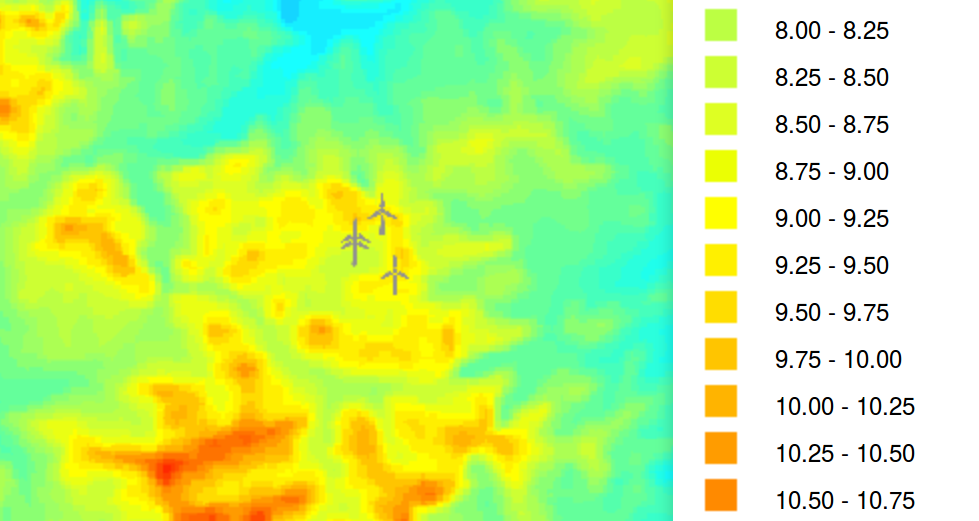
\includegraphics[width=1\textwidth]{seai_wind_atlas_kilgarvan}
  \end{center}
  \caption{Wind speed at 75m - SEAI Wind Atlas - Kilgarvan Area}

According to the SEAI Wind Atlas \cite{seai_atlas}, the area has average wind speeds at 75m height of 8 - 10 ms^-1.

% TODO: Something about wind reliability - weibull

The terrain is flat/not flat - based on what criteria.


\subsection{Access Route}
Access to Kilgarvan windfarm is off the N22. 

The first bit of electricity infrastructure visible is an Eirgrid/ESB operated substation just off the main road. This substation connects directly to the 110kV grid.

The wind farms are situated on the western side of the Derrynasaggart mountains. An access road winds from the N22 to the site. The road passes through both rocky and bog areas. Some cutting away of bog and rock was necessary to build the road. The road has a gentle incline and wide turns. Turbines were transported to the site in large sections on this road so it has a gentle incline and wide turns.
Road works were recently completed on the site to improve the access route.
% reference for transporting turbine sections
The area on the lee side of the hills is forested. Although the land is owned by the wind farm operator, Brookfield, the forestry is managed by Caoilte.


% research building roads through bogs



\section{Technology}
% TODO: Main kilgarvan site ?? Proper names?
\subsection{Wind Machines}
There are two types of wind turbine installed on the site that was visited. The Vestas V90 is a 3MW turbine. The blades are made from lightweight carbon fibre and glass fibre composite materials. The nacelle and tower are also designed to reduce weight. The light weight reduces transportation, installation and foundation costs \cite{v90-3.0}. The V90 has a rotor diameter of 90m.
Vestas \cite{v90-3.0} describe the V90 as 'a great choice for high and medium wind sites with high turbulence'. 
The V90 can be used with a variety of different tower heights, but at Kilgarvan it is mounted on a 75m tower. The V90 was originally designed for offshore use. The turbines at Kilgarvan were the first V90 turbines installed onshore.
There are XX Vestas V90 turbines on the site and they are approximately 8 years old.

The other turbine on the site is the Nordex N90. This is a 2.5MW turbine with a 90m rotor diameter. It has similar design specifications as the Vestas V90. Nordex \cite{n90} describe the N-90 as 'As an all-round turbine ... (that) can be deployed at strong-wind sites'.

Both turbines meet the IEC-1A certification. Turbines with this certification are designed for average wind speeds of 10m/s with extreme 50 year gusts of 50m/s \cite{burton_wind_2001}. The A certification means these turbines are suitable for use in areas of high turbulence.

The Noredex turbine uses an electrical pitch control system. Each turbine has battery backup for the pitch control system.

The Vestas machines use a hydraulic pitch system that does not require battery backup.

The blades on the Vestas machines appear to be swept back significantly. The Nordex blades appear straighter. There was a noticeable twist along the length of the blades. This twist is designed in to accommodate the difference in apparent wind speed along the blades.

\begin{center}
  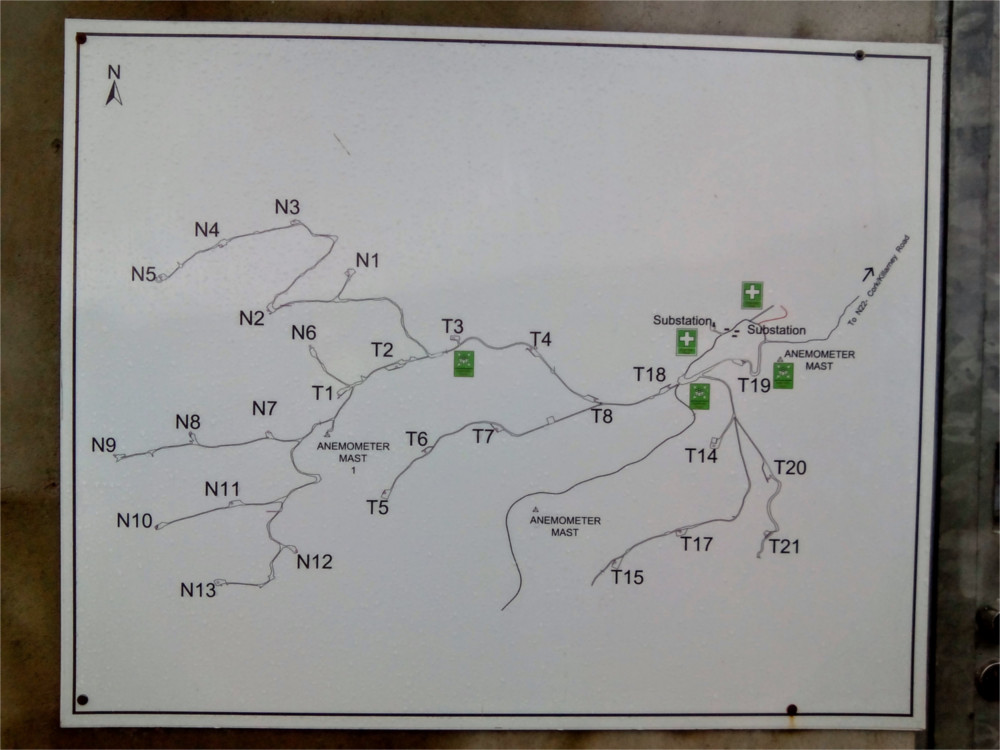
\includegraphics[width=1\textwidth]{kilgarvan_layout}
\end{center}
\caption{Layout of the wind farm. N indicates a Nordex turbine, T indicates a Vestas machine}

Some machines are in better sites than others. Some machines are located in depressions, or shadowed by the hillside if the wind is blowing in a particular direction. The power output of the turbines can vary significantly depending on their location. The worst performing machines only generate 40\% of the power as the best performers. This is taken into account at the design stage.

Each turbine has an access door at the base of the tower. Inside, there is a voltage converter, turbine control system and a ladder and lift to access the nacelle.

\subsection{Electrical Infrastructure}
The turbines generate electricity at 1000V. The voltage is stepped up to 20kV at the bottom of the turbine where it is connected to the local on-site grid. The voltage is stepped up to 110kV at the Brookfield operated substation at the top of the site.

The on-site grid between the turbines and the substation is not visible and can be assumed to use underground cables.
The Brookfield substation is connected to the ESB substation with a series of wooden and metal pylons. The pylons carry five cables - one for each phase of the 3-phase electricity being generated, one ground cable and one communications fibre optic cable.

\section{Operations and Conditions}

\subsection{Maintenance Requirements}
\paragraph{Planned Maintenance:}
Wind machines need periodic maintenance to keep them operating safely and efficiently. 
Both turbines are quite old designs and the manufactures have continued to improve the design of the machines. If possible, these improvements are applied to the turbines during maintenance.
The original design of the V90 gearbox experienced more failures. The design was improved and the gearboxes were replaced with the new design.

The maintenance period is specified by the turbine manufacturer.
Nordex machines are serviced twice per year and Vestas machines are serviced once a year. 
Maintenance is carried out by contractors who travel from site to site around the country.

Type 3 maintenance was recently completed on the Nordex machines at the Kilgarvan site. Type 3 maintenance involves replacing the battery backups and checking and tightening every bold in the turbine. During maintenance, the turbine must be stopped. Type 3 maintenance takes one week and the turbine will be down for between 8-10 hours per day.
Type 2 maintenance is less time consuming. 1 in 8 bolts will be checked and tightened. If there is any significant movement, all bolts in that turbine will be checked.

A number of inspections are carried out as part of the maintenance. The tower and blades of the turbine are inspected visually. Depending on maintenance schedule, they are inspected using high definition cameras or rope access workers. Site operators are also trialling drone aircraft inspections. Brookfield recently trialled drone inspections and compared the results to the current methods.
The engineers reported that damage to the blades is one of the common issues. A common problem is people shooting at turbine blades.

\paragraph{Unplanned Maintenance:} 
Turbines experience downtime from time to time for different reasons. One of the nearby Vestas turbines was not operating on the day of the site visit.

% TODO: Not ray's name?
While we were in the turbine, Not Ray remarked that there was a 'bearing gone' in the rotor. He could tell this because the rotor was making a different noise as it rotated. This bearing could be easily replaced from inside the nacelle and would not cause significant downtime.

Road works recently completed.

\subsection{The day we visited}
The wind speeds on the day of the visit were very variable. The average wind speed was 10m/s but it varied from 6m/s - 13m/s. 
The wind was blowing from south-south-east. The usual wind direction at this site is south-west, and the site layout is optimized for this direction.
SSE wind blows over rougher terrain than SW. This contributed to the variable conditions on the day.

The pitch of the turbine blades was constantly changing as the automatic control system attempted to get the maximum amount of power from the variable winds.
% TODO: Other name?
The Ray, one of the Brookfield engineers, estimated the turbine was operating at around 75\% capacity due to the variable winds.

At the time of the visit, all of the power being generated was being accepted by the grid. This is the usual scenario, as wind, as a renewable source, is higher in the merit order. % TODO: reference merit order.
% TODO: Explain what curtailment means better
From time to time, the grid managers will reject some wind generated power. This may be needed to ensure grid stability. This scenario is known as curtailment.

Ray is a Brookfield engineer who operates a nearby 100MW farm.
He expected higher, more consistent winds that evening. Due to the stronger winds and lower loads expected at night, Ray expected production from his farm to be curtailed to 75MW that evening. As his farm has a non-firm connection, this means there would be no compensation for the curtailment.

\subsection{A day in the life of a wind farmer}
Ray spoke about his work as an engineer on a wind farm. The work varies and there is no typical day.

\paragraph{Sub Contractors:} While one Brookfield engineer typically manages a wind farm site, contractors are frequently on site to carry out works and maintenance. On the day of our visit, a team from Vestas were leaving the site as we arrived. 

\paragraph{Liaising with Eirgrid:} An important aspect of the site engineers job is to work with the grid operator to ensure the farm is transmitting the maximum possible power to the grid.

\paragraph{Community relations:} Public relations are an important aspect of Ray's job. The public are permitted to access the lands around the turbines and the engineers will often meet with them. Horse riders regularly access the site.
Ray reported that Brookfield have a good relationship with the local community. They make significant donations to local community causes, including the GAA.

\subsection{Environmental Affects}

\paragraph{Birds:} 
Ray's farm is in a Special Area of Conservation and is a know habitat for red grouse \cite{birds}.

Wind farming can affect bird populations in the following ways:
  \begin{itemize}
    \item{Collision with turbine blades}
    \item{Displacement from habitat}
    \item{Habitat change}
    \item{Deviation in flight paths}
  \end{itemize}

Environmental consultants do regular surveys to see if there are any red grouse nesting nearby. If a nest is found near a turbine, that machine must be shut down for the duration of the nesting season.

\paragraph{Noise:} When standing directly underneath the turbine, there was a regular, swishing noise. Noise was not an obvious problem in other areas of the site. It was a blustery day and the noise of the turbines was not significantly higher than the background wind noise.
Because the wind farm is on the windward side of the mountain in a sparsely populated area, noise complaints are not an issue.

\paragraph{Skyline:} The turbines are not visible from the main road and there is no houses in the immediate area. Some of the electricity infrastructure is visible.

\paragraph{Construction:} The access road for the wind farm passes through an area of bog.

\paragraph{Drainage:} The wind farm has affected drainage on the site. Covered culverts are being trialled. % TODO: What was the problem??


\section{Conclusion}
On-shore wind farming in Ireland is a mature, well developed business. Wind farms are assets that are often sold between large, successful companies.
Wind turbines are complex machines that require careful maintenance. This maintenance is typically taken care of by the turbine manufacturers or third parties, rather than the wind farm operator. 
A well sited and managed wind farm does not have significant environmental affects. Wind farm operators can have a good relationship with local communities


%----------------------------------------------------------------------------------------
% BIBLIOGRAPHY
%----------------------------------------------------------------------------------------
\printbibliography

%----------------------------------------------------------------------------------------

\end{document}